\thispagestyle{timhieukhoahocnone}
\pagestyle{timhieukhoahoc}
\everymath{\color{timhieukhoahoc}}
\blfootnote{$^1$\text{\color{timhieukhoahoc}Viện Sinh thái và Môi trường Đông Dương.}}
\graphicspath{{../timhieukhoahoc/pic/}}
\begingroup
\AddToShipoutPicture*{\put(0,616){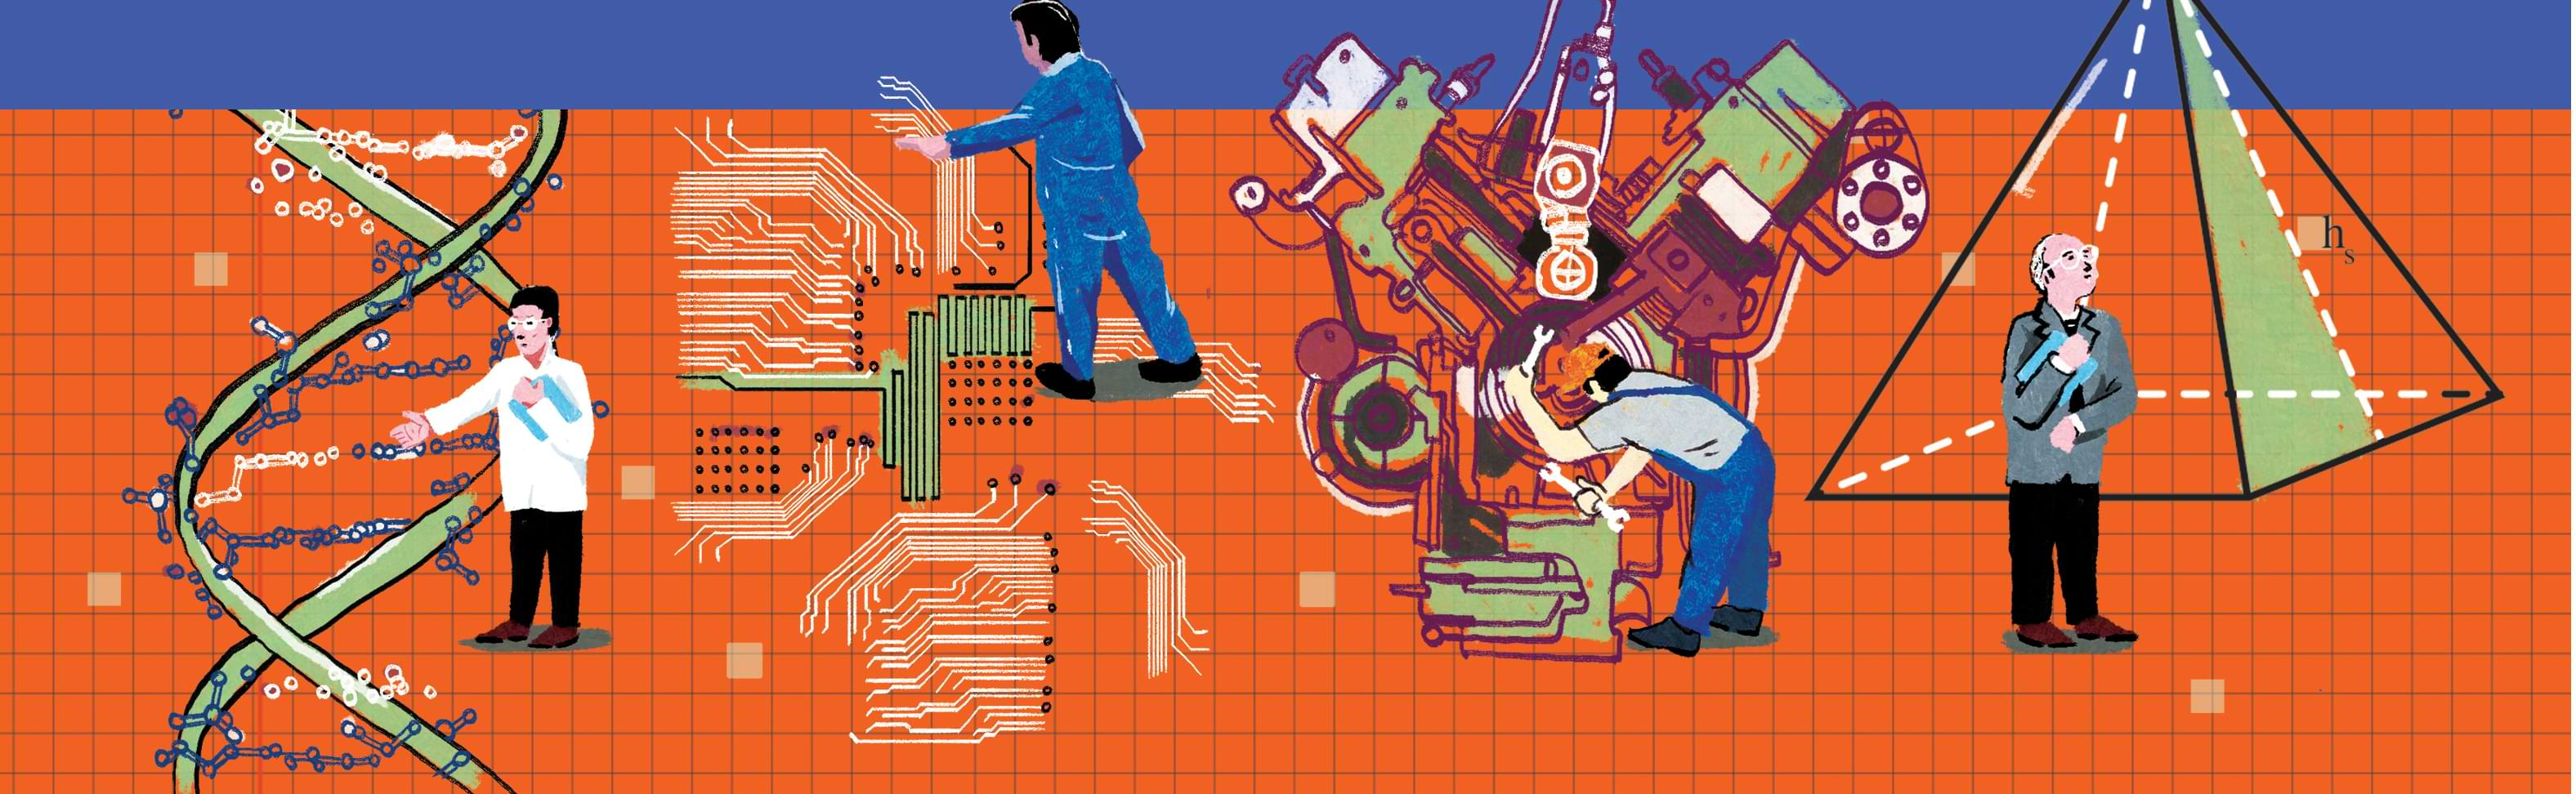
\includegraphics[width=19.3cm]{../bannertimhieu}}}
\AddToShipoutPicture*{\put(58,495){
\includegraphics[scale=1]{../tieude.pdf}}}
\centering
\endgroup
\vspace*{210pt}

\begin{multicols}{2}
	Trái đất được hình thành khi nào là một câu hỏi mà từ xa xưa con người đã sáng tạo các câu chuyện mang đậm màu sắc huyền thoại lẫn tôn giáo. Cuối thế kỷ $19$, nhiều nhà khoa học đã đưa ra các giả thuyết về bằng nhiệt hay lượng muối tích tụ ở biển. Tuy nhiên, câu trả lời chính xác chỉ xuất hiện vào giữa thể kỷ $20$ với các đo đạc đồng vị chì do phóng xạ của Clair Patterson. Quá trình này cũng giúp ông khám phá một vấn đề môi trường nghiêm trọng của thế kỷ $20$. Chúng ta hãy cùng tìm hiểu câu truyện của Patterson trong bài viết này.
	\vskip 0.1cm
	$\pmb{1.}$ \textbf{\color{timhieukhoahoc}Đường isochron và tuổi của Trái đất}
	\vskip 0.1cm
	Năm $1944$, Clair Patterson, khi vừa tốt nghiệp thạc sĩ chuyên ngành hóa học, bị bắt buộc tham gia dự án Manhattan (dự án chế tạo bom nguyên tử của quân đội Mỹ) dù ông không tình nguyện. Trong quá trình này, ông đã tiếp xúc với các thí nghiệm về các đồng vị của uranium cũng như phương pháp phổ khối lượng để đo hàm lượng các đồng vị.
	\vskip 0.1cm
	\textbf{\color{timhieukhoahoc}Đồng vị là gì?}
	\vskip 0.1cm
	Các nguyên tử của cùng một nguyên tố có số lượng proton trong hạt nhân giống nhau nhưng số lượng neutron có thể khác nhau, tạo thành các đồng vị. Ví dụ, carbon có các đồng vị với nguyên tử khối khối là $12$, $13$ và $14$ (ký hiệu là $^{12}{C}$, $^{13}{C}$ và $^{14}{C}$).
	\begin{figure}[H]
		\vspace*{-5pt}
		\centering
		\captionsetup{labelformat= empty, justification=centering}
		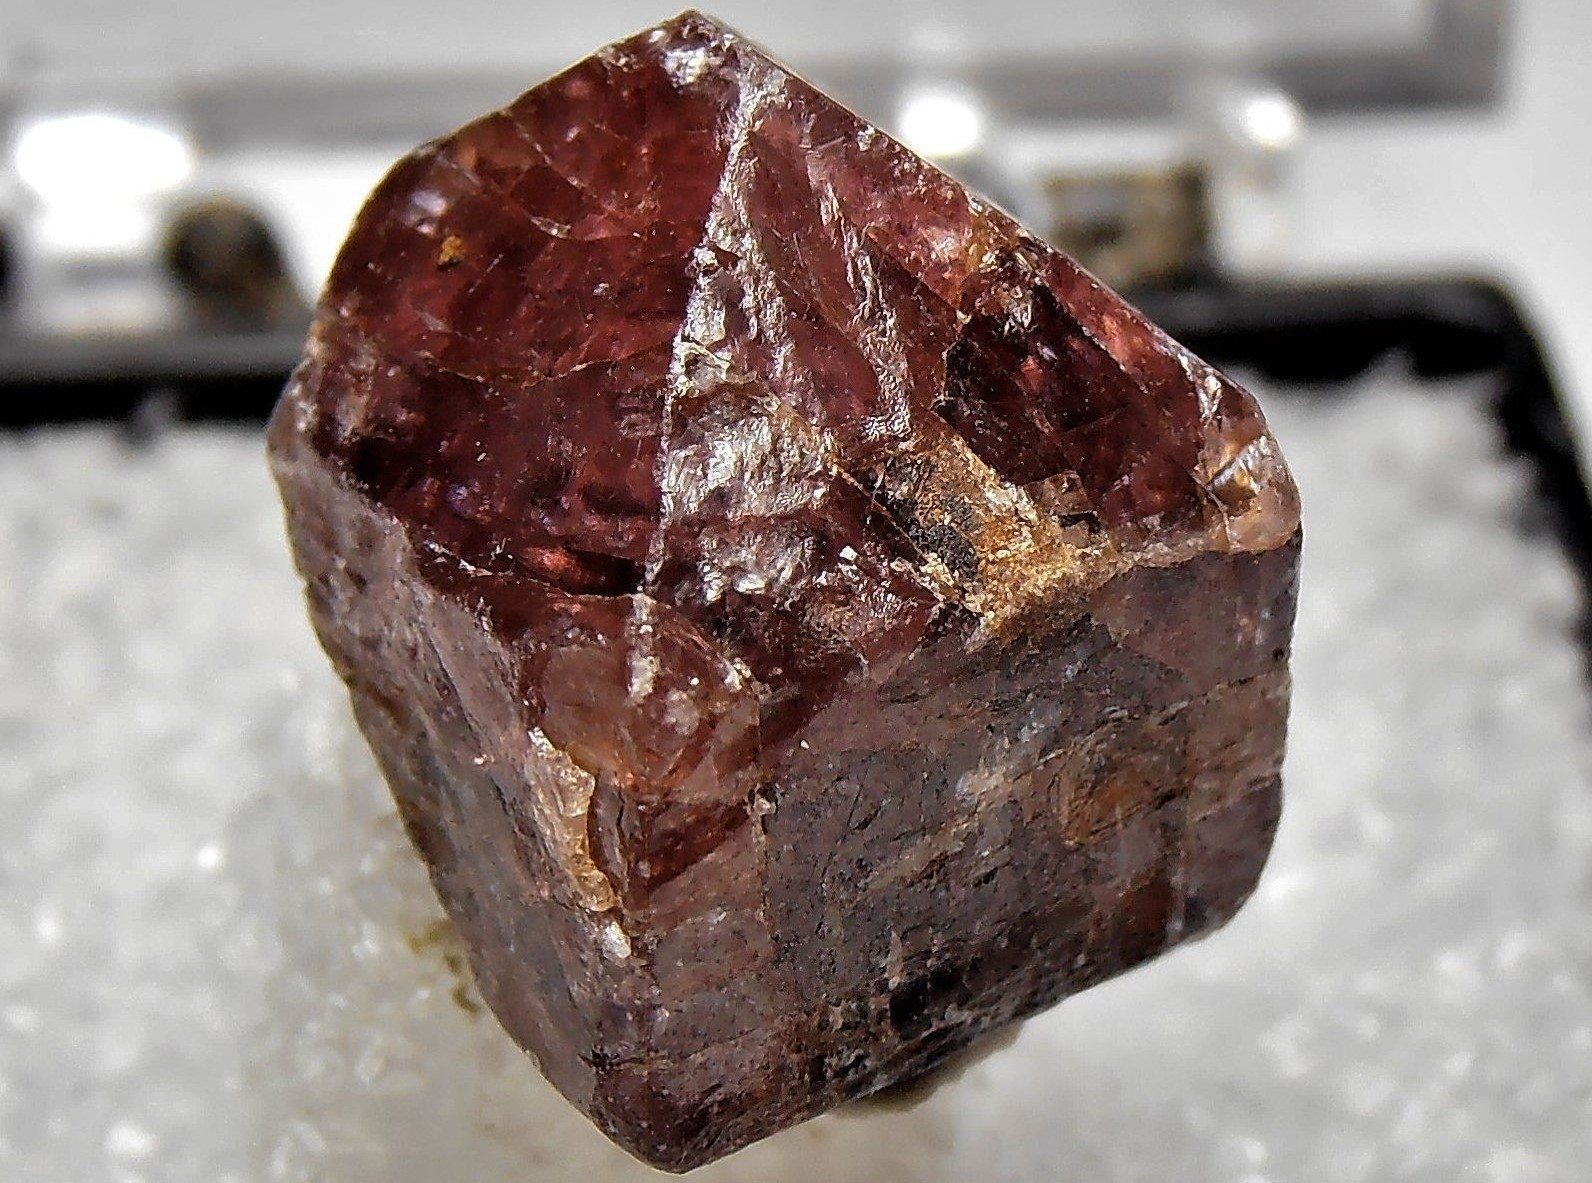
\includegraphics[width= 1\linewidth]{1}
		\caption{\small\textit{\color{timhieukhoahoc}Hình $1$. Tinh thể zircon (${ZrSiO}_4$)}}
		\vspace*{-10pt}
	\end{figure} 
	Sau chiến tranh, Patterson quay lại làm nghiên cứu sinh ở Đại học Chicago. Ở đây, ông gặp được giáo sư Harrison Brown và tham gia nghiên cứu về việc xác định tuổi của Trái đất sử dụng phép đo đồng vị phóng xạ cùng với George Tilton, một nghiên cứu sinh khác của Brown. Cả hai bắt đầu tiến hành các thí nghiệm xác định tuổi của mẫu vật với các tinh thể zircon. Các tinh thể rất nhỏ này thường xất hiện trong các loại đá núi lửa thông thường. Khi các loại đá này hình thành do magma nóng chảy đông đặc lại, các tinh thể zircon sẽ lẫn vào trong. Do cấu tạo, zirconium trong tinh thể zircon có thể được thay thế bởi uranium nên các tinh thể zirconium thường có một lượng nhỏ uranium bên trong.
	\vskip 0.05cm
	\textbf{\color{timhieukhoahoc}Phân rã phóng xạ}
	\vskip 0.05cm
	Một số nguyên tử không ổn định có thể bị phân rã thành nguyên tử khác kèm theo giải phóng một số hạt (hạt nhân helium, electron, photon). Các đồng vị phóng xạ khác nhau khi phân rã tạo thành các sản phẩm đồng vị khác nhau. Ví dụ với uranium, một chất phóng xạ phổ biến, $^{238}{U}$ phân rã thành đồng vị chì $^{206}{Pb}$ còn $^{207}{U}$ phân rã thành $^{207}{Pb}$.
	\vskip 0.05cm
	Nếu tại thời điểm ban đầu có $N_0$ nguyên tử chất phóng xạ thì số lượng nguyên tử của nó sẽ giảm theo hàm mũ theo phương trình:
	\begin{align*}
		N = N_0 e^{-\lambda t}
	\end{align*}
	với $\lambda$ là hằng số phân rã (đặc trưng cho từng đồng vị phóng xạ). Sau mỗi chu kỳ bán rã: $t_{\frac{1}{2}} = \frac{\ln 2}{\lambda}$ thì số nguyên tử sẽ giảm đi một nửa.
	\vskip 0.05cm
	Mặt khác, khi uranium phân rã theo thời gian tạo thành chì, lượng uranium trong tinh thể giảm dần còn sản phẩm chì này sẽ bị đẩy ra ngoài tinh thể. Các đồng vị chì hình thành do quá trình phân rã của uranium có nguyên tử khối khác với chì thông thường do đó nếu đo khối lượng của các đồng vị này cùng lượng uranium còn lại trong tinh thể, ta có thể xác định tuổi của tinh thể nhờ chu kỳ bán rã của uranium.
	\vskip 0.05cm
	Patterson và Tilton phải làm việc với các tinh thể zircon chỉ bé bằng đầu cây kim và đo các khối lượng nhỏ hơn $1000$ lần so với những thí nghiệm trước thời điểm đó. Những tinh thể trong các thí nghiệm được lấy từ những mẫu đá với số tuổi đã được xác định từ tuổi địa chất của chúng (vị trí trong các lớp địa tầng). Trong khi các đo đạc uranium của Tilton tiến hành thuận lới thì các số liệu đồng vị chì của Patterson không khớp với tính toán.
	\vskip 0.1cm
	Sau khi kiểm tra các tính toán với số liệu cũng như thử các kỹ thuật thí nghiệm khác nhau, Patterson phát hiện ra rằng kết quả đo lượng chì bị tăng vọt ra do môi trường thí nghiệm bị nhiễm chì từ bên ngoài. Các dụng cụ thí nghiệm, sơn tường, quần áo và tóc của người làm thí nghiệm đều bị nhiễm một lượng chì nhỏ nhưng đủ để làm hỏng các thí nghiệm của Patterson. Ông đã phải tìm cách chế tạo các phòng sạch để tránh nhiễm chì từ môi trường cũng như tiến hành tẩy chì khỏi các dụng cụ thí nghiệm. Trong quá trình này, Patterson cũng trở thành chuyên gia trong việc đo hàm lượng chì nồng độ thấp ở các vật dụng khác nhau. Các kết quả cho thấy lượng chì trong chúng cao hơn nhiều so với các kết quả trước đó.
	Khi nhận bằng tiến sĩ năm $1951$, Patterson, cùng với Tilton, đã hoàn thiện được phương pháp tính tuổi của tinh thể zircon, một trong những phương pháp chính xác định tuổi của đá trong địa chất. Trong những năm sau đó, ông tham gia chương trình sau tiến sĩ nhờ tài trợ mà Brown xin được từ Ủy ban Nguyên tử Mỹ và bắt đầu tiến hành quá trình đo tuổi của Trái đất.
	\vskip 0.1cm
	Do Trái đất luôn trải qua các quá trình biến động địa chất liên tục, các loại đá sẽ có những giai đoạn bị chôn vùi trong lớp magma dưới lòng đất và tái tạo lại khi núi lửa phun trào. Do đó, việc tìm được những mẫu đá cùng tuổi với Trái đất là rất khó. Do đó, việc xác định tuổi của Trái đất cần phải dựa vào các mẫu đá lấy từ các thiên thạch. Patterson đưa ra các giả thuyết sau: các thiên thạch và Trái đất được hình thành cùng lúc trong quá trình phát triển của hệ Mặt trời; các thiên thạch tồn tại dưới dạng hệ cô lập và kín; vào thời điểm hình thành các thiên thạch có tỷ lệ giữa các đồng vị chì giống với như Trái đất lúc đó; các thiên thạch có tỷ lệ giữa các đồng vị uranium giống với Trái đất.
	\vskip 0.1cm
	Các mẫu thiên thạch mà Patterson sử dụng gồm hai loại: thiên thạch sắt và thiên thạch đá. Các thiên thạch sắt, được coi là giống với các vật liệu hình thành lõi từ của Trái đất, khi hình thành bị mất hết uranium nên có tỷ lệ các đồng vị chì giống với thời điểm mà Trái đất hình thành. Các thiên thạch đá khi hình thành cũng có tỷ lệ các đồng vị chì như vậy nhưng do có một lượng uranium nhất định nên tỷ lệ giữa các đồng vị chì của chúng thay đổi theo thời gian. Mối liên hệ giữa các tỷ lệ đồng vị chì này được biểu diễn thông qua mô hình Holmes -- Houtermans.
	\vskip 0.1cm
	Giả sử có một hệ kín từ thời điểm $T_0$ (khi Trái đất hình thành) so với hiện tại cho đến thời điểm hiện tại ($t=0$). Tại thời điểm hiện tại, số nguyên tử các đồng vị uranium đo được trong mẫu này là  $^{238}U$ và $^{235}U$ còn số nguyên tử các chì đo được là $^{206}Pb$, $^{207}Pb$ và $^{204}Pb$.
	\vskip 0.1cm
	Tại thời điểm $t$ bất kỳ (tính ngược từ hiện tại trở về trước), ta có các phương trình phân rã phóng xạ (với $\lambda_{238}$ và $\lambda_{235}$ lần lượt là hằng số phân rã của các đồng vị uranium tương ứng):
	\begin{align*}
		&^{238}U(t) = ^{238}U_0e^{-\lambda_{238}(T_0 -t)} \tag{$1$}\\
		&^{235}U(t) = ^{235}U_0e^{-\lambda_{235}(T_0 -t)} \tag{$2$}
	\end{align*}
	Lượng các đồng vị chì cũng bằng lượng ban đầu cộng với lượng được sinh ra do phân rã (số nguyên mỗi đồng vị chì sinh ra bằng số nguyên tử của đồng vị uranium sinh ra nó bị hụt đi):
	\begin{align*}
		&^{206}\!Pb(t) \!=\! ^{206}\!Pb_0 \!+\! \left(^{238}\!U_0 \!-\! ^{238}\!U(t)\right) \tag{$3$}\\
		&^{207}\!Pb(t) \!=\! ^{207}\!Pb_0 \!+\! \left(^{235}\!U_0 \!-\! ^{235}\!U(t)\right) \tag{$4$}
	\end{align*}
	Đặt $r_1 (t)= \frac{^{206}Pb(t)}{^{204}Pb},r_2 (t)= \frac{^{207}Pb(t)}{^{204}Pb(t)}$ (lượng chì thông thường $^{204}Pb$ không thay đổi theo thời gian) và biết rằng ở thời điểm hiện tại ($t=0$), $\frac{^{235}U}{^{238}U} = \frac{1}{137,88}$ với tất cả mẫu đá trên Trái đất; sau một số biến đổi ta được:
	\begin{align*}
		\frac{r_2(t) \!-\! b_0}{r_1(t)\!-\! a_0} \!=\! \frac{1}{137{,}88} \!\cdot\! \frac{e^{\!-\!\lambda_{235}T_0}\!-\! e^{\!-\!\lambda_{235}t}}{e^{\!-\!\lambda_{238}T_0}\!-\! e^{\!-\!\lambda_{238}t}} \tag{$5$}
	\end{align*}
	với $b_0$ và $a_0$ là các giá trị của $r_2$ và $r_1$ tại $T_0$.
	\vskip 0.1cm
	Quan hệ trên cho ta liên hệ giữa $r_2$ và $r_1$ không phụ thuộc vào số nguyên tử uranium. Nó cho thấy rằng, những mẫu vật khác nhau với cùng tỷ lệ các đồng vị chì ở thời điểm ban đầu và lượng uranium ban đầu khác nhau thì đều nằm trên cùng một đường thẳng trên biểu đồ biểu diễn theo quan hệ giữa $r_2$ và $r_1$. Đường thẳng này còn gọi là đường isochron ứng với thời điểm $t$.
	\vskip 0.1cm
	Trong thí nghiệm của mình, Patterson đã tiến hành đo đạc các đồng vị chì trong $5$ mẫu thiên thạch ($2$ thiên thạch sắt và $3$ thiên thạch đá). Kết quả (công bố năm $1953$) cho thấy chúng đều nằm trên cùng một đường isochron ứng với $T_0=4,55$ tỷ năm ($t=0$ ứng với thời điểm hiện tại). Đây cũng là số liệu chính xác đầu tiên về tuổi của Trái đất. Hiện tại, số liệu của Patterson, với chu kỳ bán rã của uranium mới cập nhật, cho ta kết quả $4,48$ tỷ năm. Tỷ lệ đồng vị chì Patterson đo được trong thiên thạch sắt thu được ở Canyon Diablo (Mỹ) được sử dụng làm các giá trị cho $a_0$ và $b_0$ trong ($5$) để vẽ các đường isochron ứng với các thời điểm $t$ khác. Khi đó, mô hình Holmes -- Houtermans cũng có thể áp dụng cho các loại quặng bị mất toàn bộ uranium khi hình thành vào thời điểm $t=T$. Chúng sẽ nằm trên đường isochron ứng với thời điểm $T$ này.
	\begin{figure}[H]
		\vspace*{-5pt}
		\centering
		\captionsetup{labelformat= empty, justification=centering}
		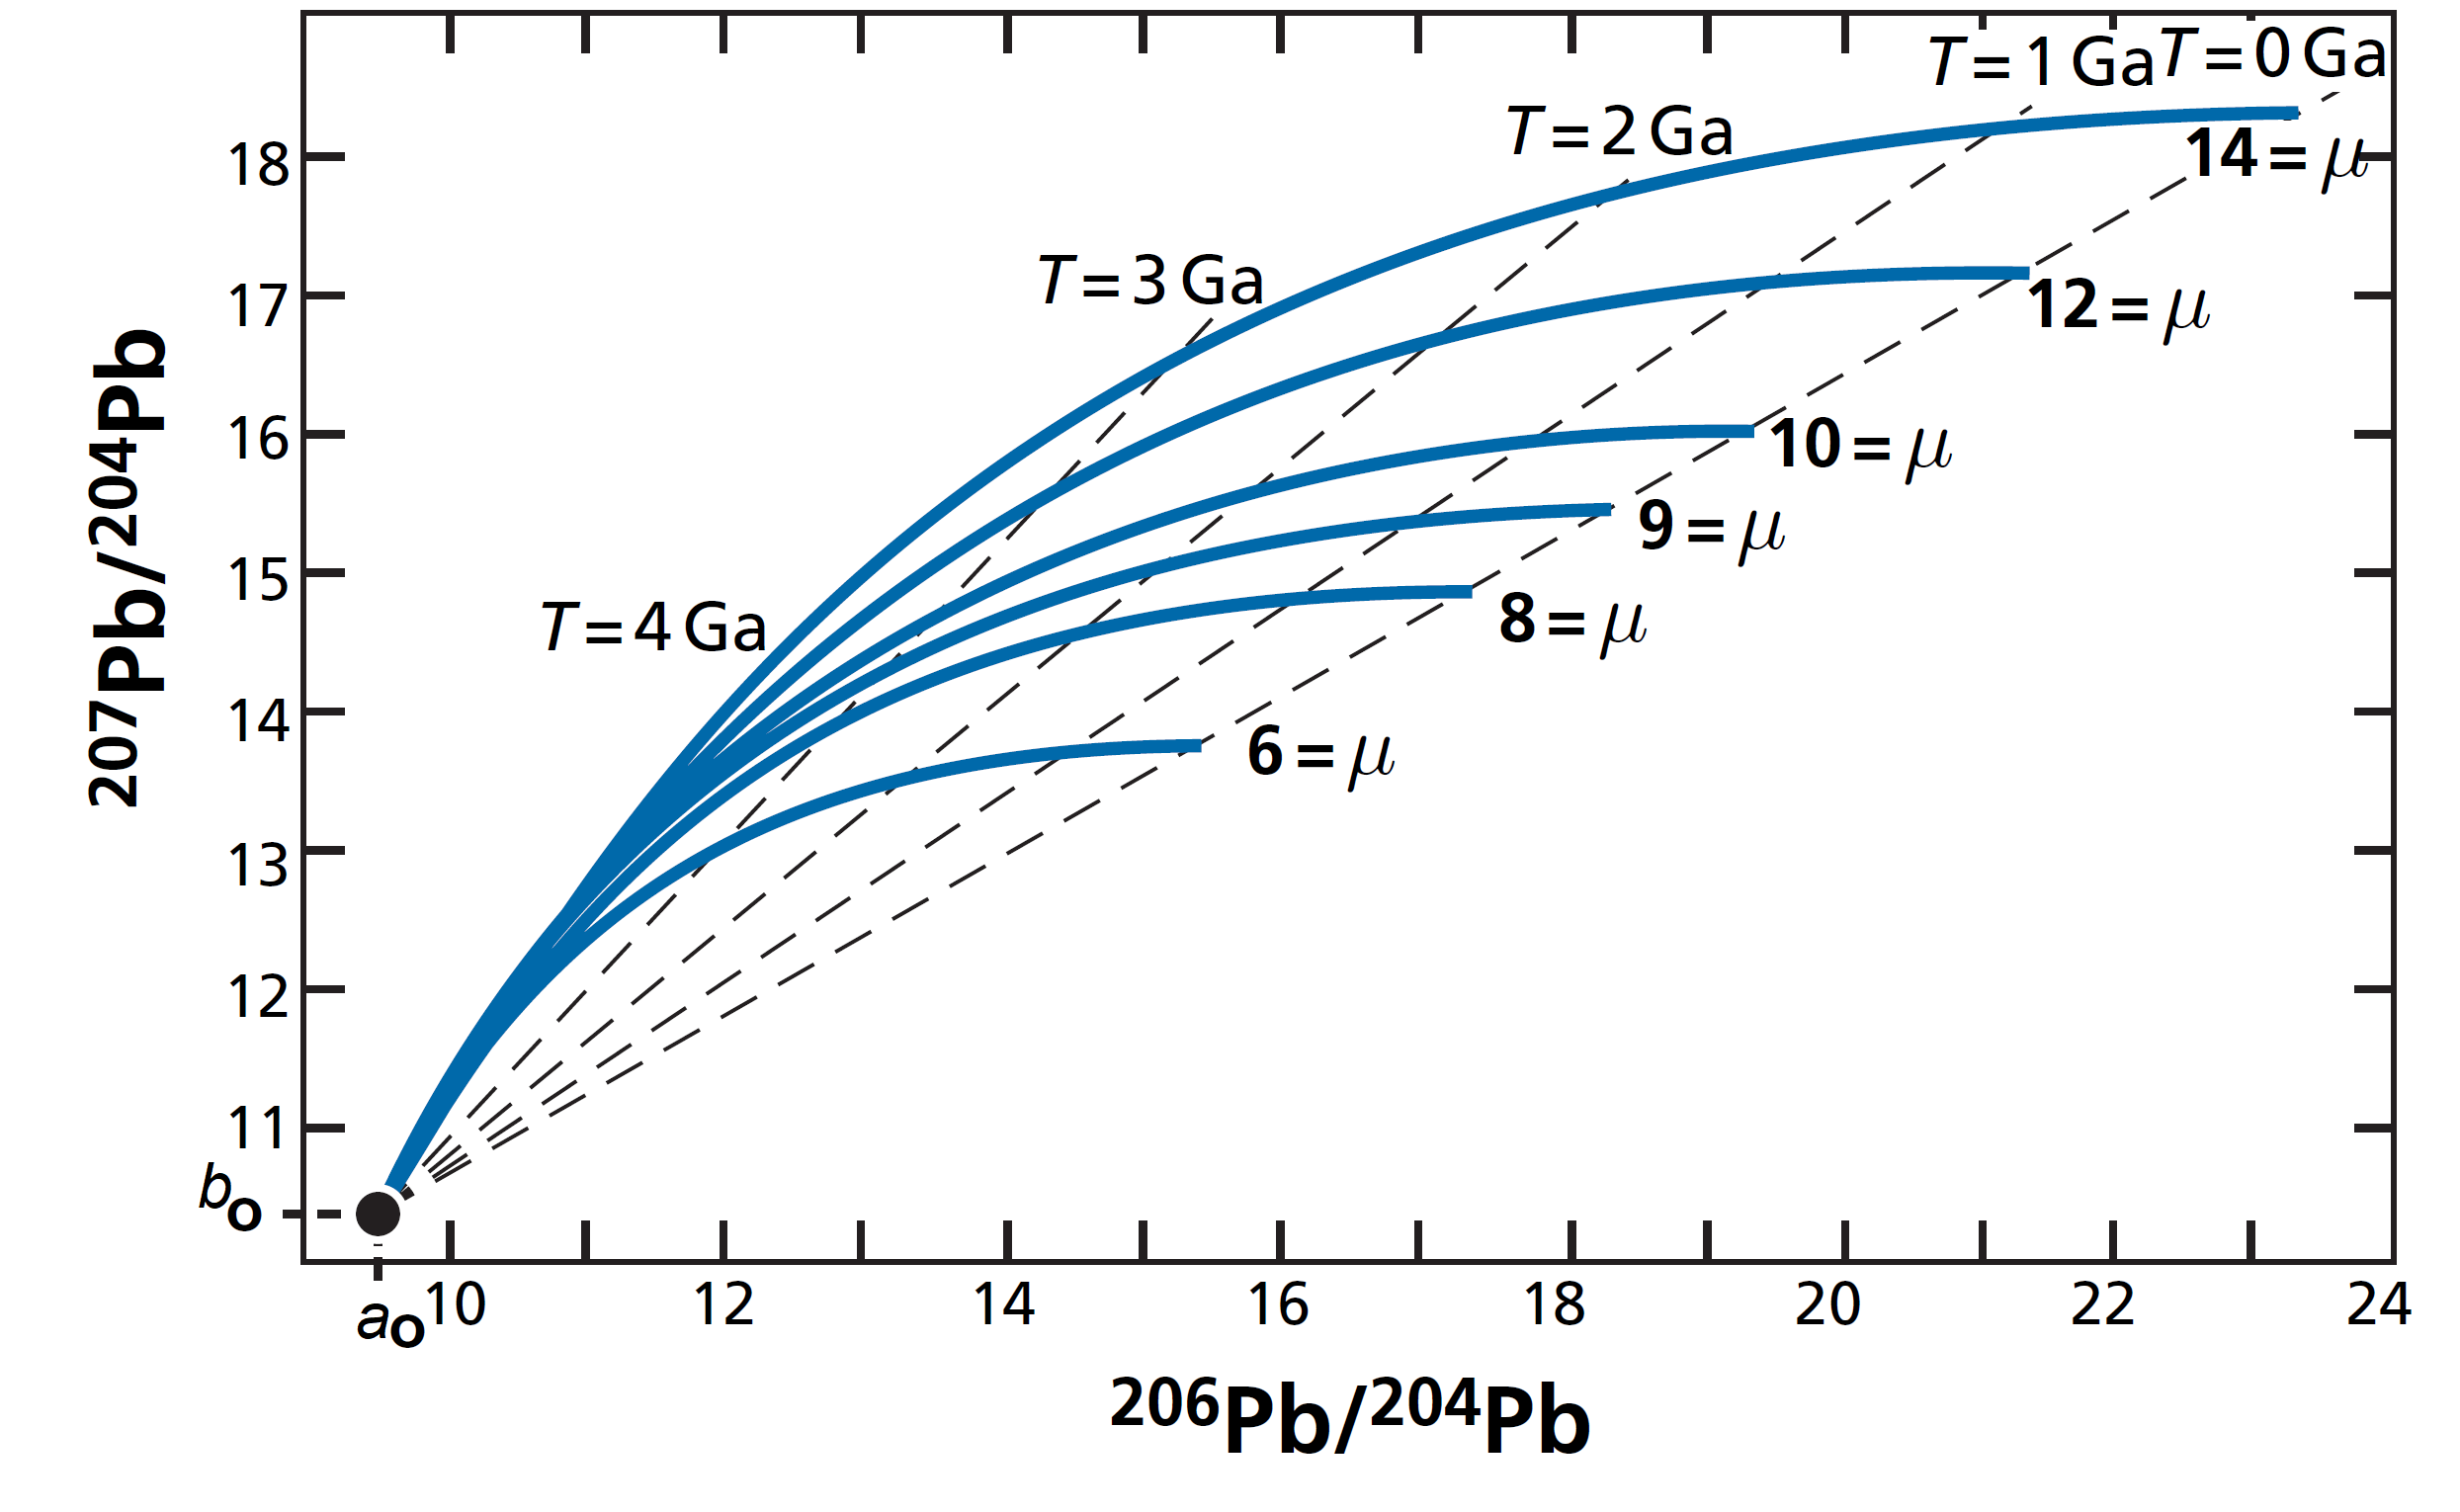
\includegraphics[width= 1\linewidth]{2}
		\caption{\small\textit{\color{timhieukhoahoc}Hình $2$. Mô hình Holmes -- Hautermans. Những mẫu đá có cùng tỷ lệ đồng vị chì ban đầu nhưng hàm lượng uranium khác nhau sẽ đi theo những đường cong khác nhau nhưng tại mỗi thời điểm, các điểm biểu diễn chúng đều nằm trên một đường isochron.}}
%		\vspace*{-5pt}
	\end{figure}	
	Cùng thời điểm với Patterson, nhiều nhà khoa học vẫn đang thử các phương pháp xác định tuổi của Trái đất sử dụng các phương pháp phân rã phóng xạ khác như kali -- argon và rubidium -- strontium. Patterson đã vượt lên trước những nghiên cứu khác do ông có thể loại bỏ các nguồn chì tạp chất khi tiến hành thí nghiệm.
	\begin{figure}[H]
		\vspace*{-5pt}
		\centering
		\captionsetup{labelformat= empty, justification=centering}
		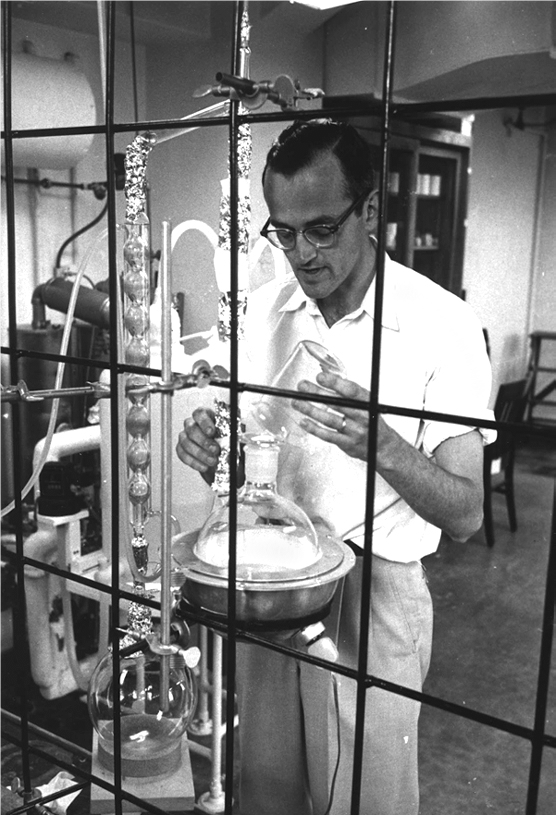
\includegraphics[width= 1\linewidth]{3}
		\caption{\small\textit{\color{timhieukhoahoc}Hình $3$. Patterson trong phòng thí nghiệm ($1952$).}}
		\vspace*{-10pt}
	\end{figure}
	\textbf{\color{timhieukhoahoc}$\pmb{2.}$ Vấn đề ô nhiễm chì}
	\vskip 0.1cm
	Tiếp theo đó, Harrison Brown lại tìm được một nguồn tài trợ mới cho các nghiên cứu của Patterson: các công ty dầu mỏ. Việc đo đạc đồng vị chị trong các mẫu trầm tích ở đáy biển có thể giúp xác định loại đá của lớp trầm tích, giúp đánh giá khả năng của sự tồn tại mỏ dầu tại vị trí khoan thăm dò. Kết quả đánh giá theo mô hình Holmes -- Hautermans cho thấy một số mẫu trầm tích dưới đáy biển cũng nằm trên cùng một đường isochron với các kết quả đo đạc với các thiên thạch.
	\vskip 0.1cm
	Tuy nhiên, các thí nghiệm lại cho Patterson thấy một vấn đề nghiêm trọng hơn khi xét đến lượng chì tích tụ trong các lớp trầm tích. Trong khi phần lớn chì ở đáy biển đến từ các hạt đất sét chảy từ các con sông ra biển, một lượng chì nhỏ hơn nhiều được hình thành do các sinh vật phù du. Chúng hấp thụ chì hòa tan trong nước biển khi còn sống và khi xác của chúng chìm xuống lớp trầm tích, các tinh thể chứa chì sẽ hình thành. Việc đo đạc lượng chì từ các tinh thể này có thể cung cấp thông tin về lượng chì trong các đại dương của Trái đất trong thời gian kéo dài hàng triệu năm.
	\vskip 0.1cm
	Cùng lúc đó, một số nghiên cứu đo đạc lượng chì ở nhiều con sông cho kết quả gấp nhiều lần so với lượng chì tích tụ ở đáy biển trong quá khứ mà Patterson đo được. Để kiểm chứng việc này, Patterson đã tiến hành các thí nghiệm lấy mẫu nước ở các độ sâu khác nhau trong lòng biển. Sau khi tiến hành các tính toán, Patterson nhận thấy một khả năng: lượng chì tăng vọt trong nước biển có thể là do nguồn chì trong không khí từ việc đốt xăng dầu. Ngay sau khi Patterson công bố bài báo về việc này, nguồn tài trợ từ các công ty dầu mỏ lập tức chấm dứt!
	\vskip 0.1cm
	\textbf{\color{timhieukhoahoc}Xăng pha chì}
	\vskip 0.1cm
	Năm $1921$, Thomas Midgley và Charles Kettering, khi đó đang làm việc ở General Motors, phát hiện rằng việc cho phụ gia chì tetraethyl (TEL) vào trong xăng sẽ giúp loại bỏ hiện tượng nhiên liệu cháy trước khi động cơ đánh lửa, giúp công suất của các động cơ ô tô tăng lên. Năm $1923$, một loạt vụ ngộ độc chì với biểu hiện rối loạn thần kinh dẫn đến tử vong ở nhiều nhà máy sử dụng TEL xảy ra. Midgley và các công ty lớn làm mọi cách để trấn an dư luận về sự an toàn của sản phẩm này và các biện pháp an toàn được tiến hành để giảm thiểu phơi nhiễm của công nhân ở các nhà máy. Mặt khác, Charles Kettering thuê Robert Kehoe, một chuyên gia về độc chất học, để sản xuất các công bố khoa học chứng tỏ rằng phơi nhiễm chì từ xăng không ảnh hưởng đến sức khỏe cộng đồng trong suốt vài chục năm.
	\begin{figure}[H]
		\vspace*{-5pt}
		\centering
		\captionsetup{labelformat= empty, justification=centering}
		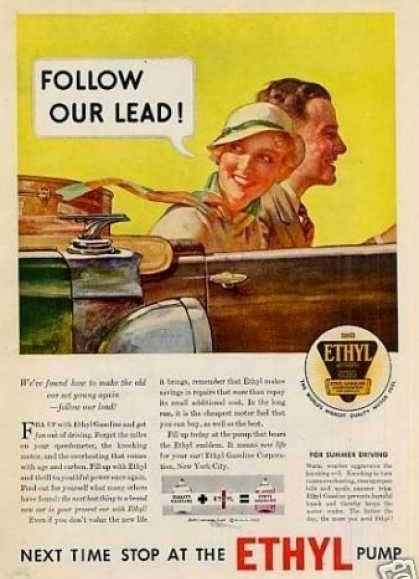
\includegraphics[width= 1\linewidth]{4}
		\caption{\small\textit{\color{timhieukhoahoc}Quảng cáo xăng pha chì năm $1933$. Các tập đoàn lớn như General Motors, Dupont và Standard Oil tiến hành quảng cáo rầm rộ cho sản phẩm này đồng thời với việc cố gắng phủ định tác hại của nó.}}
		\vspace*{-10pt}
	\end{figure}
	Patterson vẫn không hề nản chí và tiếp tục tìm các nguồn tài trợ cũng như các hợp tác khoa học để tiếp tục điều tra về vấn đề ô nhiễm chì. Các mẫu tuyết lấy từ các độ sâu khác nhau gần Bắc Cực và New Zealand mà Patterson thu được cho thấy nồng độ chì tăng từ $200$ đến $300$ lần so với $300$ năm trước đó. Việc đo lượng chì rất nhỏ này được tiến hành với các kỹ thuật cải tiến từ thời kỳ Patterson làm việc với Harrison Brown. Patterson cũng bắt đâu xét đến khía cạnh y học của chì. Trong giai đoạn tham gia dự án chế tạo bom nguyên tử, Patterson đã biết đến các thí nghiệm về quá trình đào thải barium phóng xạ ở sinh vật. Tỷ lệ barium phóng xạ trong sữa của con bò thí nghiệm thấp hơn rất nhiều lần so với tỷ lệ barium trong cỏ mà nó ăn do phần lớn bị cơ thể đào thải. Do đó, Patterson cũng tò mò về hiệu quả đào thải chì của cơ thể. Trong thời gian làm giáo sư thỉnh giảng ở đại học MIT, ông thường xuyên đến thư viện Y khoa của đại học Havard. Các dữ liệu cho thấy cơ thể người không đào thải chì một cách hiệu quả. Các kiến thức về địa chất giúp Patterson có một cái nhìn mới về quá trình này. Tỷ lệ chì/calcium trong xương người gần với tỷ lệ này trong các mẫu đá trong tự nhiên! Cũng có nghĩa là, phần lớn lượng chì được hấp thụ vào xương cùng với calcium.
	\vskip 0.1cm
	Patterson đã có một hành trình đi khắp thế giới để đo nồng độ chì từ các nguồn khác nhau: đại dương, lõi băng ở các cực Trái đất, động thực vật. Ông còn tiến hành đo nồng độ chì trong các xác ướp cổ xưa ở Peru. Các đo đạc của Patterson cho thấy mức độ chi được coi là “bình thường” trong các nghiên cứu y khoa lúc đó thật sự cao hơn rất nhiều lần so với trạng thái tự nhiên. Ông cũng tham gia các nghiên cứu khảo cổ học cho thấy việc khai thác các mỏ bạc thời Hy Lạp và La Mã cổ đại đã gây ra các giai đoạn tương ứng với hàm lượng chì trong khí quyển Trái đất cao hơn nhiều so với trước đó.
	\vskip 0.1cm
	\textbf{\color{timhieukhoahoc}Ô nhiễm chì thời La Mã}
	\vskip 0.1cm
	Hiện nay vẫn có nhiều tranh cãi về mức độ ảnh hưởng của chì đối với xã hội La Mã. Nhiều đường ống dẫn nước trong các thành phố La Mã được làm bằng chì. Do chưa có đường mía, người La Mã nấu quả nho trong các nồi chì (do các nồi đồng sẽ có mùi tanh) để làm các chất tạo ngọt, đặc biệt khi uống với rượu vang. Đã có giả thuyết được đưa ra cho rằng mức độ nhiễm độc chì cao ở tầng lớp cai trị dẫn đến các câu chuyện trong lịch sử về sự điên khùng của các hoàng đế La Mã, góp phần dẫn đến sự sụp đổ của đế quốc. 
	\vskip 0.1cm
	\textbf{\color{timhieukhoahoc}$\pmb{3.}$ Giảm thiểu ô nhiễm chì}
	\vskip 0.1cm
	Những nghiên cứu của Patterson và nhiều nhà khoa học khác là tiền đề cho các phong trào đấu tranh giảm thiểu ô nhiễm chì, đặc biệt là xăng pha chì trong thập niên $1970$. Nhiều nghiên cứu tiếp theo đã khẳng định tác hại của xăng pha chì vẫn luôn bị hệ thống công nghiệp tìm cách phủ định thông qua các nghiên cứu được tài trợ. Tuy vấp phải sự chống đối từ các tập đoàn lớn, quá trình giảm chì trong xăng bắt đầu ở Mỹ vào năm $1983$. Năm $1986$, Nhật Bản là nước đầu tiên cấm hoàn toàn xăng pha chì. Năm $2001$, Việt Nam cũng ngừng sử dụng xăng pha chì. Năm $2021$, Algeria là nước cuối cùng tiến hành chuyển sang sử dụng xăng không chì.
	\vskip 0.1cm
	Chì trong sơn cũng là một nguồn gây ngộ độc chì cho con người. Chì thường được cho vào sơn để giảm ăn mòn và giúp cho sơn khô nhanh hơn. Nó đặc biệt nguy hại với trẻ nhỏ vì chúng thời chơi gần mặt đất và dễ tiếp xúc với sơn tường. Nhiều nước, trong đó có Việt Nam, cũng đã có các quy định về việc quản lý lượng chì trong sơn. Ở nhiều nước khác, chì vẫn chưa được loại bỏ khỏi sơn do chi phí chuyển đổi công nghệ.
	\vskip 0.1cm
	Các nỗ lực giảm thiểu chì đã có hiệu quả đáng kể. Ở Mỹ, nồng độ chì trung bình trong máu trẻ em năm $2016$ giảm $95\%$ so với năm $1978$. Tuy nhiên, với những người đã bị phơi nhiễm chì với lượng lớn từ trước đó, hậu quả lâu dài thực sự vẫn rất khó đánh giá. Một nghiên cứu mới đây ước tính có $170$ triệu người Mỹ đang sống bị phơi nhiễm chì ở mức độ cao ở thời kỳ trẻ em và mức độ sụt giảm trí tuệ trung bình do chì là khoảng $2{.}6$ điểm IQ. Ảnh hưởng của phơi nhiễm chì với các bộ phận khác trong cơ thể cũng là một đề tài được các nghiên cứu y học quan tâm.
	\vskip 0.1cm
	Hiện nay, chì vẫn xuất hiện trong đời sống trong nhiều sản phẩm như ắc quy chì, mỹ phẩm, thiết bị điện tử, ... Phơi nhiễm chì do tiếp xúc trực tiếp hoặc từ chì trong đất và nước ngầm vẫn là một vấn đề đáng quan tâm.
	\vskip 0.1cm
	\textbf{\color{timhieukhoahoc}$\pmb{4.}$ Lời kết}
	\vskip 0.1cm
	Tại Mỹ, xăng pha chì chỉ bị cấm hoàn toàn vào năm $1996$, nhiều tháng sau khi Patterson mất. Câu chuyện của Clair Patterson cho thấy sự cần thiết của các nghiên cứu khoa học độc lập để tránh sự mất kiểm soát của công nghệ khi chỉ chạy theo mục đích lợi nhuận. Bản thân Patterson cũng là một tấm gương của một nhà khoa học nghiêm túc với ý thức về sự đóng góp của các nghiên cứu cho lợi ích chung của cộng đồng.
	\begin{figure}[H]
		\vspace*{5pt}
		\centering
		\captionsetup{labelformat= empty, justification=centering}
		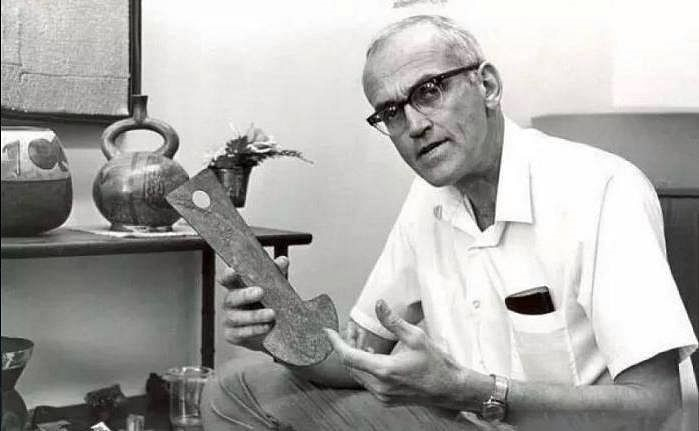
\includegraphics[width= 1\linewidth]{5}
		\caption{\small\textit{\color{timhieukhoahoc}Clair Patterson ($1922 - 1995$).}}
		\vspace*{-10pt}
	\end{figure}
	\textbf{\color{timhieukhoahoc}Tài liệu tham khảo}
	\vskip 0.1cm
	[$1$] Allgegre, C. ($2008$). Isotope Geology. Cambridge University Press.
	\vskip 0.1cm
	[$2$] Patterson, C. ($1956$). Age of meteorites and the earth. \textit{Geochimica et Cosmochimica Acta}, $10$, $230-237$.
	\vskip 0.1cm
	[$3$] Patterson, C. ($1965$). Contaminated and Natural Lead Environments of Man. \textit{Environmental Health: An International Journal.}
\end{multicols}